\section{Analysis}
From the result, can be seen that the most common gene that show up in the cluster is GO:0005515 which has function of protein binding. (See section Result).

Every heatmap of every cluster can be see at figure \ref{pic:cluster-1}, \ref{pic:cluster-2}, \ref{pic:cluster-3}, \ref{pic:cluster-4} and \ref{pic:cluster-5}. At figure \ref{pic:cluster-5} the heatmap have the most red color (sorry if the capture not good quality) compare with other figure. In chapter results, this cluster (cluster 5) have the offten gene ontology id GO:0005515, with the main basic function of protein binding.

Refered to \href{http://amigo.geneontology.org/amigo/term/GO:0005515}{http://amigo.geneontology.org/amigo/term/GO:0005515}, this GO "protein binding" is part of molecular function. This also has an another name or id, GO:0045308, and synonyms characteristic are:  protein amino acid binding, alpha-2 macroglobulin receptor-associated protein activity, protein degradation tagging activity, protein tagging activity, and protein folding chaperone. The graphs view of this GO can see at figure \ref{pic:gv-go}. This GO has a subset (actually we are not known what is it) are:
\begin{itemize}
	\item gosubset\_prok
    \item goslim\_plant
    \item goslim\_pir
    \item goslim\_candida
    \item goslim\_aspergillus
    \item goslim\_chembl
\end{itemize}

\begin{figure}[htbp]
	\centering
	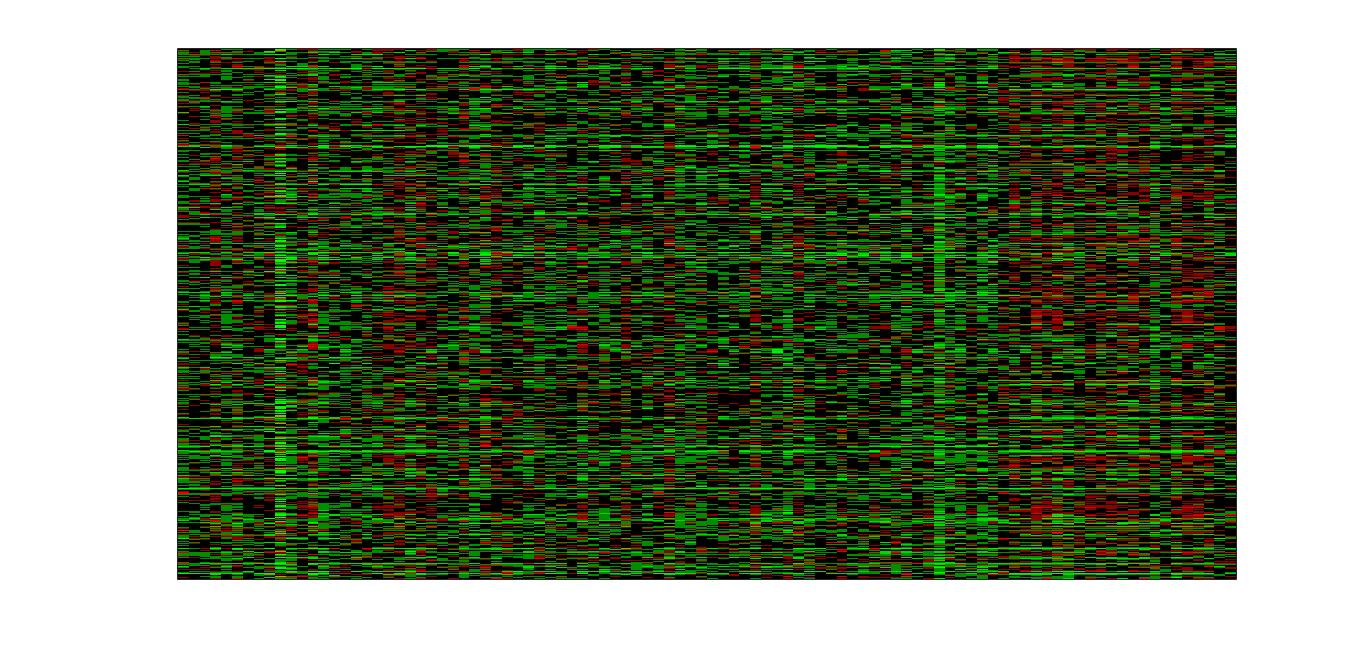
\includegraphics[height=6.5cm]{analisis/raw.jpg}
	\caption{Heatmap raw data}
	\label{pic:raw}
\end{figure}

\begin{figure}[htbp]
	\centering
	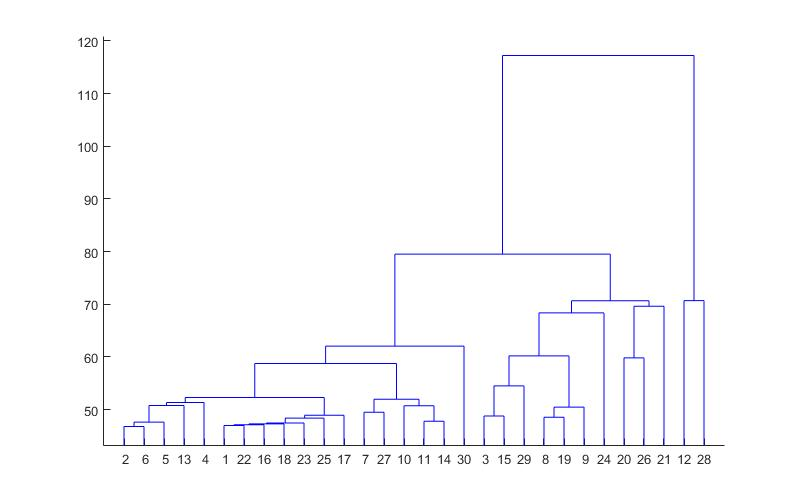
\includegraphics[height=6.5cm]{analisis/dendogram.jpg}
	\caption{Dendogram}
	\label{pic:dendo}
\end{figure}

\begin{figure}[htbp]
	\centering
	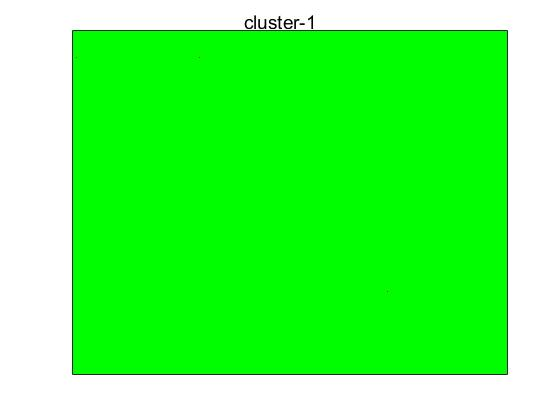
\includegraphics[height=6.5cm]{analisis/cluster-1.jpg}
	\caption{Heatmap cluster-1}
	\label{pic:cluster-1}
\end{figure}

\begin{figure}[htbp]
	\centering
	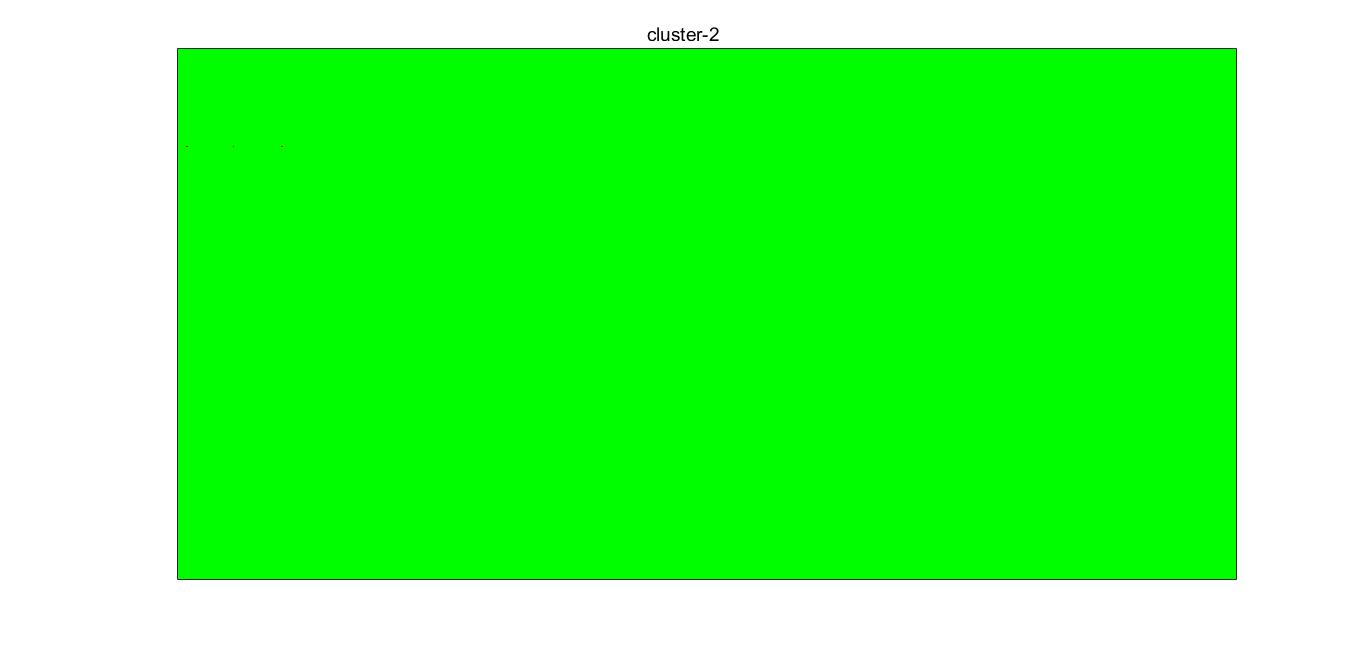
\includegraphics[height=6.5cm]{analisis/cluster-2.jpg}
	\caption{Heatmap cluster-2}
	\label{pic:cluster-2}
\end{figure}

\begin{figure}[htbp]
	\centering
	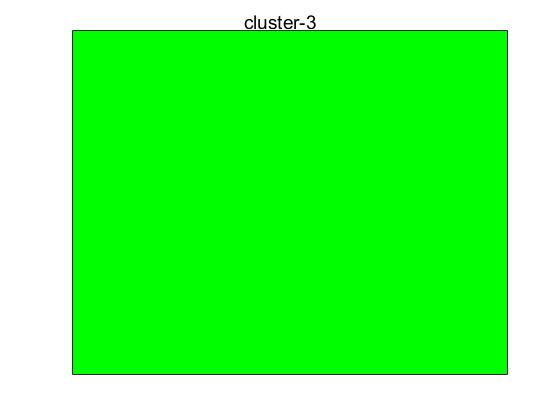
\includegraphics[height=6.5cm]{analisis/cluster-3.jpg}
	\caption{Heatmap cluster-3}
	\label{pic:cluster-3}
\end{figure}

\begin{figure}[htbp]
	\centering
	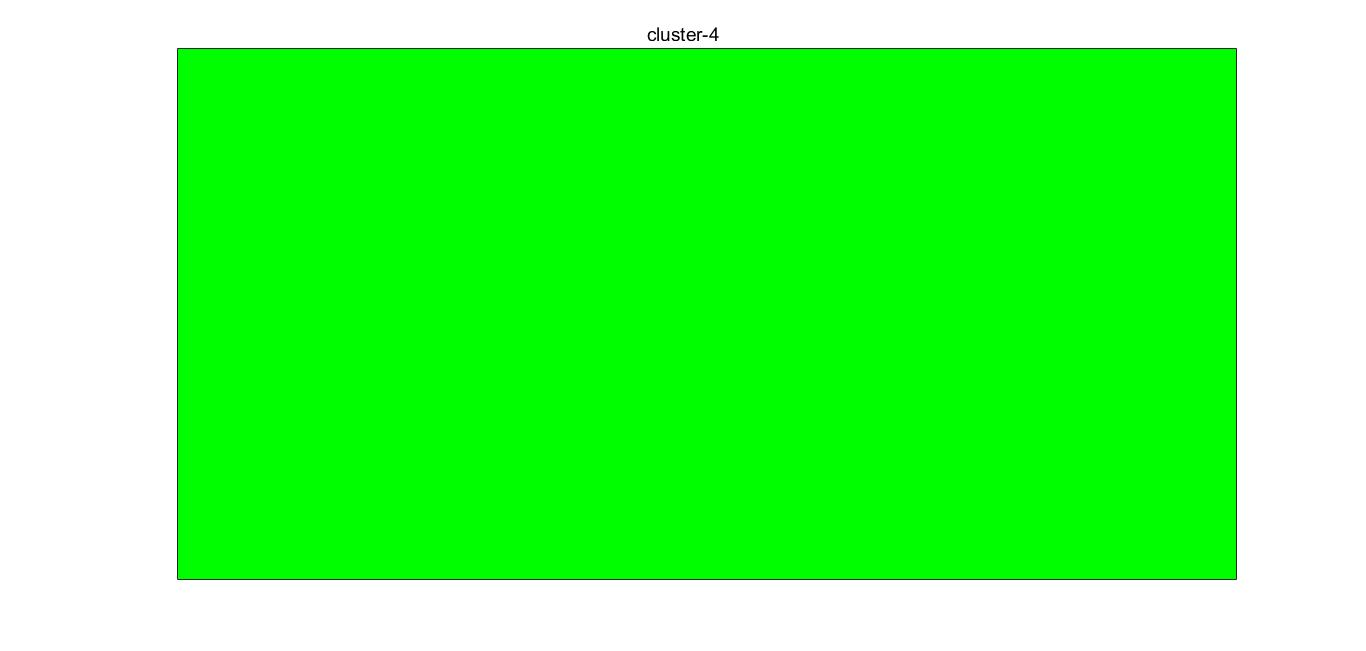
\includegraphics[height=6.5cm]{analisis/cluster-4.jpg}
	\caption{Heatmap cluster-4}
	\label{pic:cluster-4}
\end{figure}

\begin{figure}[htbp]
	\centering
	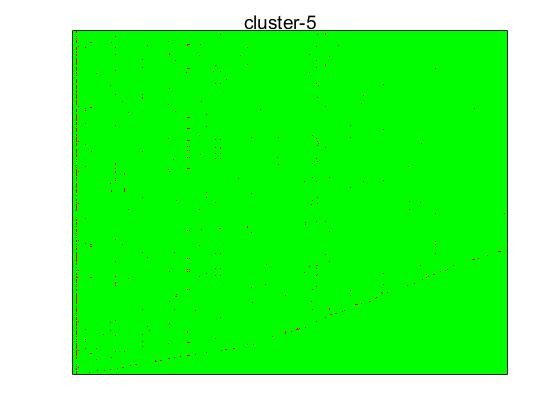
\includegraphics[height=6.5cm]{analisis/cluster-5.jpg}
	\caption{Heatmap cluster-5}
	\label{pic:cluster-5}
\end{figure}

\begin{figure}[htbp]
	\centering
	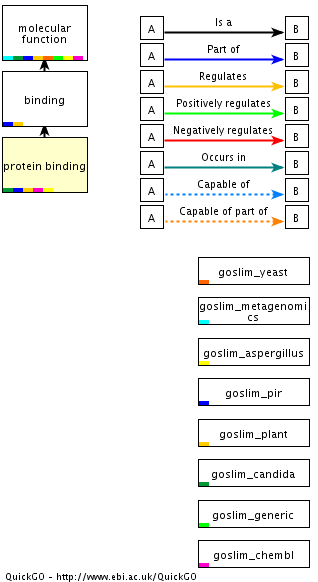
\includegraphics[height=13cm]{analisis/visualize.png}
	\caption{Graphs view of GO:0005515}
	\label{pic:gv-go}
\end{figure}
